\documentclass[12pt,a4paper,titlepage]{article}
\usepackage[utf8]{inputenc}
\usepackage{polski}
\usepackage{listings}
\usepackage{graphicx}
\usepackage{xcolor}
\usepackage{minted}
\makeatletter
\newcommand{\linia}{\rule{\linewidth}{0.4mm}}
\renewcommand{\maketitle}{\begin{titlepage}
    \vspace*{1cm}
    \begin{center}\small
    Politechnika Wrocławska\\
    Wydział Elektroniki\\
    Urządzenia cyfrowe i systemy wbudowane 1
    \end{center}
    \vspace{3cm}
    \noindent\linia
    \begin{center}
      \LARGE \textsc{\@title}
         \end{center}
     \linia
    \vspace{0.5cm}
    \begin{flushright}
    \begin{minipage}{7cm}
    \textit{\small Autor:}\\
    \normalsize \textsc{\@author} \par
    \end{minipage}
    \vspace{5cm}

     {\small Wtorek, 7\textsuperscript{30}-10\textsuperscript{15} TP}\\
        Dr inż. Dariusz Caban
     \end{flushright}
    \vspace*{\stretch{6}}
    \begin{center}
    \@date
    \end{center}
  \end{titlepage}%
}
\makeatother
\author{Justyna Skalska, 225942\\
        Piotr Pawelski, 218370}
\title{Sprawozdanie nr 2\\
\large(Port szeregowy RS232)}

\begin{document}
\maketitle

\section{Wstęp}
Celem laboratorium było zaprojektowanie układu odbierającego dane z portu RS232 i przesyłającego odebrane dane z powrotem do nadawcy, a także przetestowanie go przy użyciu dostarczonego programu oraz wybranego terminala\\\\
Następnym zadaniem było dodanie do już zaprojektowanego układu opóźnienia oraz modyfikacja fragmentu odpowiadającego za odesłanie wprowadzonych przez użytkownika danych. Pojedynczy znak podany na wejściu miał zostać podzielony na dwie części (starszą i młodszą), które miały zostać wyświetlone w kodzie ASCII.\\\\
Programem wykorzystanym do wykonania zadania jest ISE Design Suite.

\section{Przebieg zajęć}
Zajęcia rozpoczęliśmy od zapoznania się z budową schematami modułu nadajnika oraz odbiornika portu RS232. Następnie zaimportowaliśmy oba moduły do naszego projektu i stworzyliśmy schemat prostego układu wysyłającego odebrane wcześniej dane w niezmienionej postaci.

\begin{figure}[H]
\centering
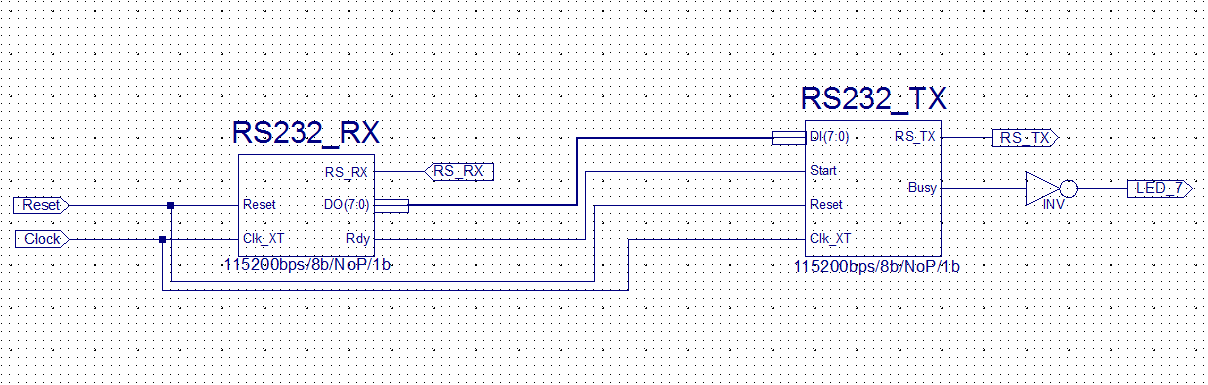
\includegraphics[angle=90,height=20cm]{rs232.png}
\caption{Schemat układu}
\label{fig:schemat}
\end{figure}

\begin{itemize}
    \item \textbf{Clock} to wejście układu odpowiadające za dostarczenie sygnału zegara,
    \item \textbf{Reset} to wejście układu odpowiadające za sygnał resetujący,
    \item \textbf{Start} rozpoczyna operację nadawania bajtu pobieranego z \textbf{DI} i ustawia sygnał \textbf{Busy} = 1
    \item \textbf{Clk\_XT} to generator kwarcowy sygnału zegarowego,
    \item \textbf{RS\_RX} odbiera bajty z portu szeregowego,
    \item \textbf{RS\_TX} wysyła bajty do portu szeregowego,
    \item \textbf{Rdy} sygnalizuje zakończenie odbioru bajtu poprzez pojawienie się a nim jedno-taktowego impulsu,
    \item \textbf{DO} to wyjście z odbiornika portu RS232,
    \item \textbf{DI} to wejście do nadajnika portu RS232,
    \item \textbf{Busy} to sygnał zajętości nadajnika (impulsy \textbf{Start} są ignorowane, gdy równy 1)
\end{itemize}

Kolejnym etapem było wygenerowanie plików VHDL oraz .jed (używany do programowania mikroprocesorów). Następnie przesłaliśmy nasz program na płytkę, gdzie udało nam się uzyskać poprawne echo danych wysłanych do portu RS232.

\section{Wnioski}
Podczas laboratoriów mogliśmy zapoznać się z podstawami tworzenia odbierania i nadawania danych poprzez port szeregowy RS232 oraz ze sposobem importu modułów do programu ISE Design Suite.\\\\
Niestety nie udało nam się wykonać drugiej części zadania. Największym problemem okazało się stworzenie opóźnienia, dzięki któremu układ wysyłałby obie części wczytanego znaku z zadaną przerwą. Udało nam się podzielić znak na bity młodsze i starsze, jednak nie zakodowaliśmy ich przy użyciu ASCII.
\end{document}